\documentclass[12pt,a4paper]{article}
\usepackage[utf8]{inputenc}
\usepackage{graphicx}
 \usepackage{datetime}
\usepackage{hyperref}
 \usepackage{biblatex} 
\addbibresource{myBib.bib}

\title{Recreating the Tokyo Railway Network with the Ant Colony Optimisation Algorithm}
\author{Gordon Tang}
\newdate{date}{18}{2}{2021}
\date{\displaydate{date}}
\setlength{\parskip}{1em}
\renewcommand{\baselinestretch}{1.2}
\DeclareUnicodeCharacter{0301}{\'{e}}

\begin{document}
\maketitle
\newpage  
\tableofcontents
\newpage  
\section{Abstract}
      
This project attempts to create the Tokyo Railway Network ~\cite{top_secret_word} with a biologically inspired algorithm called Ant Colony Optimisation (ACO) algorithm to optimise a route between cities. I applied the Travelling Salesman problem and it showed that the shortest path can be achieved.

\section{Introduction}

The Ant Colony Optimisation (ACO) was first made in ~\cite{stargazer} to model the way ants find the shortest path to a food source. The mechanism relies on a colony of ants and the pheromone hormone. Pheromone is laid on the ground based on a multitude of factors, such as distance and quality of the food source. Each ant agent starts by building their path towards a food source based on pheromone on the ground and randomness. Once the ant successfully reach the food source, it returns home while laying down pheromone hormones that signals other ants. Over time, ants converge on a path which is believed to be a good estimation for the optimal path between the home and the food. The ACO algorithm has show promising use cases to dynamic optimisation problems, NP problems and networking problems. 

The Tokyo Railway Network paper demonstrated the intelligence of a single celled organism called "slime mould". It showed that a slime mould is able to create a network between nearby food sources that optimises for fault tolerance and transport efficiency. This network shows an uncanny similarity to networks built by real world engineers. The researchers have identified several key phases of the slime mould's way of creating such a network. Key points are that it begins with a search phase over a large area, attempting to size up its environment. The next phase is the network creation phase where it slowly goes from a circular shape to an intricate network between food sources.

My project attempts to recreate this slime mould intelligent phenomenon with the Ant Colony Optimisation algorithm. I begin by using JavaScript to create a 2D grid, simulating a plot of land. A few points on the grid are marked as food sources. Next, I exhaustively search the grid starting from the centre and spreading out radially which outputs a set of coordinates. Next, I use Python to translate the set of points into a weighted graph. Next, I apply the ACO algorithm to find an optimal path between all nodes.

\section{Analysis}
\subsection{Analysis of method}
Using JavaScript to mark points of interest is a good way of visually showing the search process. Analysing with Python is good because you are not limited to the browser for computation. This allows for more scaling in the future.

Do not use randomness in the search phase. My idea was to simulate real ant agents cluelessly explore its environment but this is very inefficient and unreliable especially when scaling the grid area.

JavaScript has a weird bug that I cannot pin point. It could be the fault of the P5.js JavaScript graphics library I used, but what I thought were distinct ant agents were not really distinct as data was somehow shared despite encapsulating private variables.

I was not able to find a suitable network creation algorithm that can optimise for fault tolerance like real slime moulds. If you look at the experimental images in that paper, you see ``bridges'' between V-shaped edges. I have no clue how to implement that. The mathematical model presented in that paper looks at flow rate and tube diameter as determinants of keeping or removing a certain edge but it failed to realise the "bridging" phenomenon.
 
\subsection{Analysis of code and its result}
All code and figures can be found on my GitHub. \url{https://github.com/coffeeboost/Ant-Colony-Optimisation}

\begin{figure}[h]
   \centering
   \textbf{Pheromone levels against time}
   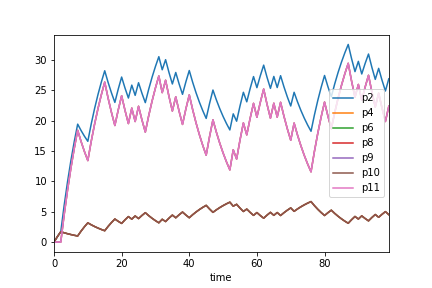
\includegraphics[width=\linewidth]{notEverything.png} 
   \caption{Plot of levels of pheromone on edges against time. (Only edges that had pheromone at the end was plotted) The up and down pattern is due to the random nature of this algorithm which could favour an alternate path many times. But the upward trend on p2, p11 and p10 show that optimal paths are generally preferred. The brown line represents the final edge back to the source point, a reason pheromone levels is so low can be seen from the paths taken by ants. Most changes in ant's path occurs on the second last step.}
   \label{fig:he_who_shall_not_be_named}
\end{figure}

\begin{figure}[h]
   \centering
   \textbf{Weighted graph in my code}
   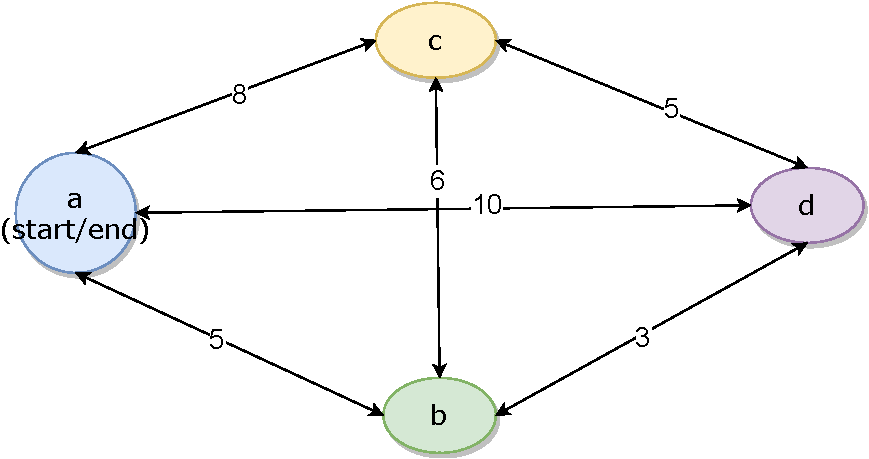
\includegraphics[width=\linewidth]{diagram.pdf} 
   \caption{According to my hand calculations, the shortest path is A-C-D-B-A for a length of 21, which is followed by A-D-B-C-A for a length of 24, and the remainder routes for a length of 26. My results converged on two paths, A-C-B-D-A and A-C-D-B-A, favouring the latter since it contained more pheromone on the last edge. This is evidence that my algorithm managed to find the most optimal solution.}
   \label{fig:i_am_voldemort}
\end{figure}

\section{Conclusions and further work}
I have applied the Travelling Salesman Problem and the Ant Colony Optimisation algorithm and attempted to recreate the Tokyo Railway Network as slime moulds have done so in a lab setting. I learned a lot about the process of research thanks to Professor Alan Tsang.

Future work can finish my incomplete code of translating coordinates to a weighted graph in a scalable manner. More research is needed for creating an algorithm that can create an actual web like network that can also exhibit "bridge" like phenomenon.

\printbibliography[heading=bibintoc]

\end{document}